\newpage
\section{\texorpdfstring{A k-matroid partíciós probléma -- MPP\textsubscript{$k$}}
		 {A k-matroid partíciós probléma}}
			 
Adott $k$ darab $M_i = (E, F_i),$ ahol $i={\overline{1,k}}$ matroid. A kérdés,
hogy a matroidok összege ($\vee_{i=1}^{k}M_i$) a szabad matroidot ($E,2^E$) adja
e? Másképp megfogalmazva előáll e az alaphalmaz $E$ az $\cup_{i=1}^{k} E_i$ alakban,
ha $\forall i$-re $E_i \in F_i$. Feltehető, hogy az $E_i$ halmazok diszjunktak, így 
egy partíciós problémához jutotunk.

\vspace{0.4cm}
\emph{MPP$_k$ P-beli probléma.}
\vspace{0.4cm}

MPP$_k \in$ NP, mert ha a feladatnak van megoldása, az egy tanú, amely lineáris időben
ellenőrizhető. MPP$_k \in$ coNP, mert ha a feladatnak nem létezzik megoldása, akkor
adhatunk rá egy $X \subseteq E$ halmazt, ami biztosan összefüggő az összegben, azaz 
$\sum r_i (X) < |X|$.



\subsection{Algoritmikus megoldás}

Most adunk erre egy algoritmust amely megoldja a feladatott, ehez kiindul üres
halmazokból és addig bőviti azokat amig uniójuk $E$ nem lesz. Ha egy adott
pontnál nem bővithető tovább egyik halmaz sem, akkor az lesz a  keresett ellen
példa, ami bizonyitás arra, hogy a matroidok nem partíciónálhatók.

\begin{figure}[htbp]
\caption{Példa, hogy a mohó algoritmus miért nem működik: 
		  $E_1 = \{2\}$, $E_2 = \{3\}$ állapotban nem tudunk újabb élt 
		  belevenni egyik halmazba sem. Egy jó partícionálás peddig a 
		  $E_1 = \{ 1 \}$, $E_2 = \{ 2, 3 \}$ felosztás.}
\label{fig:MPPMohoNem}
\centering 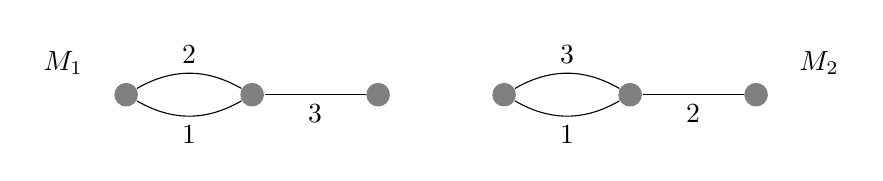
\begin{tikzpicture}[scale=0.8]
  \tikzset{ p/.style={circle,white,fill=gray,inner sep=0pt,minimum size=0.3cm},
  }
  \node[circle, fill=white] (M1) at (-3,0.5)   {$M_1$};
  \node[p] (1) at (-2,0)   {};
  \node[p] (2) at (0, 0)     {}; 
  \node[p] (3) at (+2,0)   {};
  
  \node[circle, fill=white] (M2) at (9,0.5)   {$M_2$};
  \node[p] (4) at (4,0)   {};
  \node[p] (5) at (6, 0)     {}; 
  \node[p] (6) at (8,0)   {};
  
  % the connection between the dots
  \draw[bend left,-]  (1) to node [midway, above] {$2$} (2); 
  \draw[bend left,-]  (2) to node [midway, below] {$1$} (1);
  \draw[-]  (2) to node [midway, below] {$3	$} (3);
  
  \draw[bend left,-]  (4) to node [midway, above] {$3$} (5); 
  \draw[bend left,-]  (5) to node [midway, below] {$1$} (4);
  \draw[-]  (5) to node [midway, below] {$2$} (6);
\end{tikzpicture} 
\end{figure}

Az algoritmus egy $n+k$ pontú segédgráfal dolgozik ($|E|=n$ csúcs a halmazoknak
és $k$ csúcs a particióknak), tehát $V' = E \cup \{p_1, p_2, \ldots, p_k\}$. A
gráf éleit definiáljuk mint $(\overrightarrow{xy}) \in E'$ ahol:

\begin{figure}[htbp]
\caption{Segéd gráf}
\label{fig:MPP_graf}
\centering 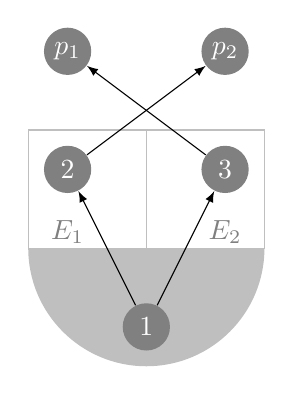
\begin{tikzpicture}[scale=1]
  \tikzset{ p/.style={circle,white,fill=gray,inner sep=0pt,minimum size=0.6cm},
  }
  \draw[lightgray] (0,0) rectangle(1.5,1.5);
  \draw[lightgray] (0,0) rectangle(-1.5,1.5);
  \node[circle,gray, fill=white] (E1) at (-1,0.2)   {$E_1$};
  \node[circle,gray, fill=white] (E2) at (+1,0.2)   {$E_2$};
  \path[fill=lightgray] (-1.5,0) arc [start angle=180, delta angle=180, radius=1.5];
  
  \node[p] (1) at (0,-1)   {$1$};
  \node[p] (2) at (-1,1)   {$2$};
  \node[p] (3) at (+1,1)   {$3$};
  \node[p] (p1) at (-1,2.5)   {$p_1$};
  \node[p] (p2) at (+1,2.5)   {$p_2$};
     
  \draw[-latex]  (1) -- (2);
  \draw[-latex]  (1) -- (3);
  \draw[-latex]  (2) -- (p2);
  \draw[-latex]  (3) -- (p1);
  
\end{tikzpicture} 
\end{figure}


\begin{itemize}
  \item  $\begin{rcases}
  x \in E \\
  y = p_i  \\
  x \not \in E_i\\
  E_i \cup  \{x\}  \in  F_i \end{rcases}
  \parbox[t]{11cm}{Egy ilyen él azt jelenti, hogy $x$-et hozzávehetjük $E_i$-hez
   a függetlenség megsérétése nélkül ($\overrightarrow{xp_i}$ -- az ábra felsõ
  részen a $p_i$-kbe mutató élek).}$
  \item $\begin{rcases}
  x,y \in E \\
  x \not\in E_i, y \in E_i\\
   E_i \cup \{x\} \not\in F_i,\\ 
   E_i \cup \{x\} - \{y\} \in F_i
  \end{rcases} \parbox[t]{10cm}{Egy ilyen él azt jelenti, hogy $x$-et
  hozzávehetjük $E_i$-hez, ha $y$-t elhagyjuk belöle ($\overrightarrow{xy}$ --
  az ábra alsó részén lévõ élek).}$
\end{itemize}

\begin{enumerate}
    \setcounter{enumi}{-1}
    \item $\forall~i~E_i = \emptyset$ kezdeti állapot ($i=\overline{1,n}$). Erre
    igaz, hogy $E_i \in F_i$.
    \item Keressük meg a legrövidebb irányított utat $E-\cup_{i}E_i$--ből
    $\left\{ p_1, \cdots, p_k \right\}$--ba.
    
    \item Ha létezik irányított út akkor ez meghatároz egy módosítás-sorozatot,
    hogy melyik $E_i$-t hogyan kell módosítanunk. Az út utolsó éle egy $p_j$-be
    megy, a többi $E$-beli elemek között, vagyis összesen 1-gyel növeljük
    $E_i$-k elemszámát.  Ha egy {\it legrövidebb} ilyen út mentén javítunk,
    akkor bizonyítható, hogy $E_i$-k a módosítások után függetlenek maradnak (mi
    nem bizonyítjuk).
    \item Különben megállunk, nemleges a válasz, és a tanú $X$ az $E- \cup Ei$--ből
    irányított úton elérhető pontok halmaza.
\end{enumerate} 

Lássuk be, hogy az algoritmus által megadott nemleges tanú valobban egy jó
ellenpélda, indirekten. Tehát:
\[ 
|X| \sum_{i=1}^k |X \cap E_i| = \sum_{i=1}^k r_i(X \cap E_i) = \sum_{i=1}^k r_i(X) 
\]

$r_i(X) \leq r_i(X \cap E_i)$ mert ha $r_i(X) > r_i(X \cap E_i)$  lenne akkor
(F$_3$) miatt $X \cap E_i$ kiegészíthetõ lenne egy $u \in X - E_i$ elemmel úgy,
hogy $F_i$-ben továbbra is független legyen. Ugyanakkor $r_i(X) \geq r_i(X \cap
E_i)$ triviális, tehát $\forall i$-re $r_i(X \cap E_i) = r_i(X)$.

\begin{figure}[htbp]
\caption{A halmazok}
\label{fig:MPP_halm}
\centering 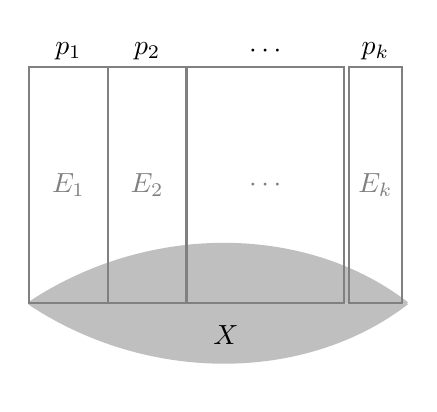
\begin{tikzpicture}[scale=1]
  \tikzset{ p/.style={circle,black,fill=white,inner sep=0pt,minimum size=0.6cm},
  }
    \draw[line width=1pt, lightgray, fill=lightgray] 
            (-0.5,-1.5) .. controls (1,-0.5) and (3,-0.5) .. (4.3,-1.5);
    \draw[line width=1pt, lightgray, fill=lightgray] 
            (-0.5,-1.5) .. controls (1,-2.5) and (3,-2.5) .. (4.3,-1.5);
  \node[p, fill=lightgray] at (2,-1.9) {$X$};
            
  \node[p] at (0,1.7) {$p_1$};
  \node[p] at (1,1.7) {$p_2$};
  \node[p] at (2.5,1.7) {$\cdots$};
  \node[p] at (3.9,1.7) {$p_k$};
  
  \node (rect) at (0,0) [gray,draw,thick,minimum width=1cm,minimum height=3cm] {$E_1$};
  \node (rect) at (1,0) [gray,draw,thick,minimum width=1cm,minimum height=3cm] {$E_2$};
  \node (rect) at (2.5,0) [gray,draw,thick,minimum width=2cm,minimum height=3cm] {$\cdots$};
  \node (rect) at (3.9,0) [gray,draw,thick,minimum width=1,minimum height=3cm] {$E_k$};
  
\end{tikzpicture} 
\end{figure}

Tehát $(X \cap E_i) \cup \{u\} \in F_i$, ezért:

\begin{itemize}
  \item vagy $E_i \cup \{u\} \in F_i$, ekkor $u \rightarrow p_i$ él be lenne
  húzva a gráfba és mivel $u$ elérhetõ $E - \bigcup_i E_i$-bõl ($X$ definíciója
  miatt), ezért $p_i$ is, tehát nem álltunk volna meg, ellentmondás.
  \item vagy $E_i \cup \{u\} \not\in F_i$, akkor van benne kör, ez a kör csak
  olyan lehet, ami $E_i-X$-be belemetsz (mivel ha $X$-ben lenne az egész kör,
  akkor $(E_i \cup \{u\})\cap X = (X \cap E_i) \cup \{u\}$ is összefüggõ lenne,
  de nem az). Legyen a körnek egy $E_i-X$-beli eleme $v$, ekkor $E_i \cup \{u\}
  - \{v\}$ független (mert független + 1 elemû halmazban csak egy kör lehet, ha
  ezt megszüntetjük, újra független lesz), tehát lenne $u \rightarrow v$ él a
  gráfban. Ez ellentmondás, mert akkor $v$ $X$-beli lenne.
\end{itemize}

Mindkét eset ellentmondás, tehát $r_i(X) = r_i(X \cap E_i)$, így $X$ tényleg jó
tanú arra, hogy nincs jó partíció.

\subsection{2-matroid-metszet probléma}

Adott $k$ matroid ($M_i=(E,F_i)$, ahol $i=\overline{1,k}$) és egy p egész szám.
A kérdés, hogy létezzik e $F_i$--nek legalább $p$ méretű közös eleme?

Az így megfogalmazott probléma $k=2$--re MMP$_2$ komplexitása P--beli.
MPP$_k$--ra már belátuk, hogy $P$--beli, MMP$_2$-őt meg megfogalmazhatjuk mint a
$M_1 \vee M_2^*$ összeg szabad matroid e?
